\documentclass{article}
\usepackage[utf8]{inputenc}

\title{Dropout: A Simple Way to Prevent Neural Networks from Overfitting}
\author{}
\date{}

\usepackage{natbib}
\usepackage{graphicx}
\usepackage{amsmath}
\usepackage[left=2.5cm,right=2.5cm,top=1cm,bottom=1.25cm]{geometry}
\usepackage{hyperref}
\usepackage{float}
\usepackage[export]{adjustbox}



\hypersetup{colorlinks=true,urlcolor=blue}
\pagenumbering{gobble}

\begin{document}

\maketitle

\section*{Link}
\href{https://www.cs.toronto.edu/~hinton/absps/JMLRdropout.pdf}{Dropout} 

\section*{Summary}
\begin{itemize}
    \item Dropout refers to dropping out units randomly from neural network. When a unit is dropped out, its temporarily removed from the network along with all its incoming and outgoing connections.
    \item The best way to regularize a fixed sized model is to average the predictions of all possible hyperparameters. But training such ensemble of models is hard and also not practical to use them at test time. Dropout prevents overfitting and provides a method for approximately combining many different neural network models efficiently.
    \item Applying dropout to a neural network amounts to sampling a thinned network from it(Figure 1). A neural network with $n$ units can be seen as a collection of $2^n$ possible thinned networks. These networks all share weights so the total number of parameters is still $O(n^2)$. For each training iteration a new thinned network is sampled and trained. So dropout can seen as a way of training a collection of $2^n$ thinned networks with extensive weight sharing.   
    \begin{figure}[H]
        \centering
        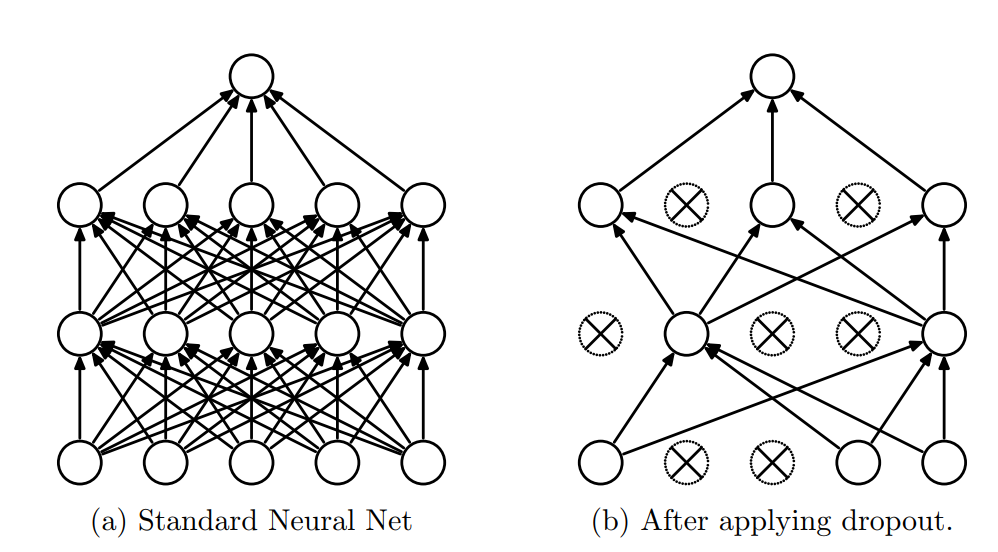
\includegraphics[scale=0.5]{dropout_model.PNG}
        \caption{Dropout neural net model}
        \label{fig:Figure 1}
    \end{figure}
    \item At test time a single neural net is is used without dropout. If a unit is retained with probability $p$ during training, the outgoing weights of that unit are multiplied by $p$ during test time. This ensures that for any hidden unit the expected output is same as the actual output at test time. 
    \item When neural networks are trained without dropout, hidden units form complex co-adaptation to achieve the target i.e. they learn to work \textit{together} to minimize the loss. So the mistakes of some units may be mitigated by others during training. But during test time on novel data if some units don't work well the entire network is more likely to fail. Dropout forces each unit to learn robust features on its own without relying on other units because it has to work with random subset of the network on each iteration. 
    \item Using dropout gives superior performance in terms of generalization error in a wide variety of tasks including vision, speech recognition, document classification, computational biology. The result on MNIST obtained with and without dropout across different architectures can be seen in Figure 2.  
    \begin{figure}[H]
        \centering
        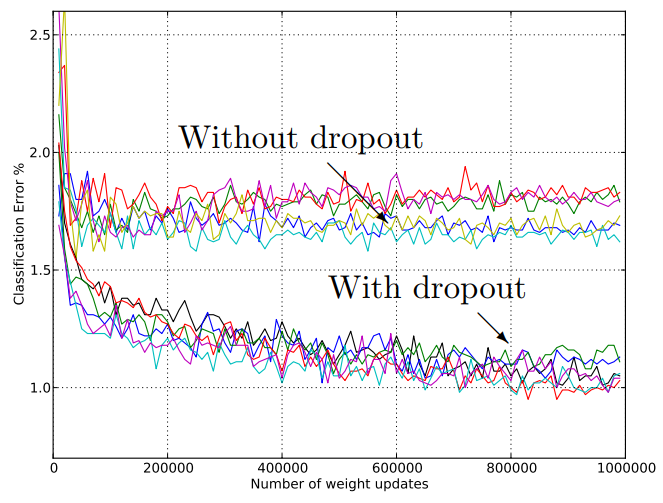
\includegraphics[scale=0.6]{performance_mnist.png}
        \caption{Test error rates of different architectures on MNIST}
        \label{fig:Figure 2}
    \end{figure}
    \item The improvement obtained in text classification task was much smaller than vision and speech recognition task.
    \item The activations in the hidden units become sparse in the presence of dropout.
    \item The optimum value for dropout rate for a wide variety of task was close to $0.5$. If we keep number of units $n$ fixed too low value of $p$ can reduce performance. Too high value of $p$ may cause overfitting. 
    \begin{figure}[H]
        \centering
        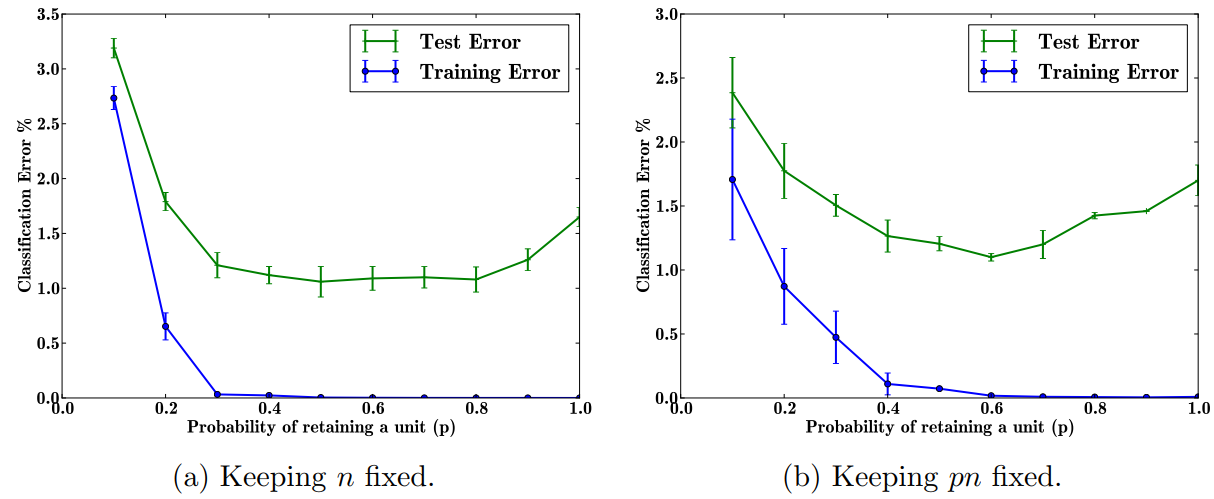
\includegraphics[scale=0.5]{dropout_rate.png}
        \caption{Effect of changing dropout rates}
        \label{fig:Figure 3}
    \end{figure}
    \item For extremely small dataset dropout does not give any improvements. As the size of the data is increased the gain from dropout increases up to a point and then decreases.
    \begin{figure}[H]
        \centering
        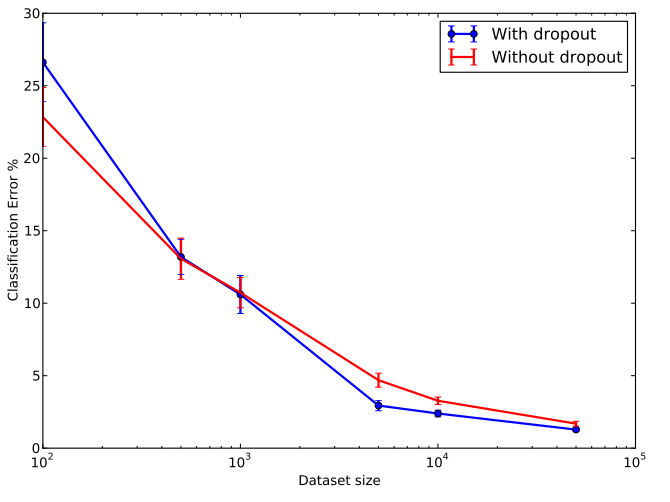
\includegraphics[scale=0.5]{dataset_size.png}
        \caption{Effect of dataset size}
        \label{fig:Figure 3}
    \end{figure}
    \item Some practical considerations for training dropout neural networks
    \begin{enumerate}
        \item If a standard neural net having $n$ units is optimal for a task, a dropout neural net should have at least $n/p$ units. For example if we use $p=0.5$ we should double the number of units.
        \item Using high learning rate and momentum significantly speed up training when using dropout.
        \item max norm regularization should be used in conjunction with high learning rate to prevent network weights to grow very large. The typical value for norm constant $c$ range from 3 to 4.
        \item The dropout rate for hidden units should be in the range of $0.5$ to $0.8$. This should be higher for input units typically 0.8.
    \end{enumerate}

\end{itemize}

\end{document}
